%%%%%%%%%%%%%%%%%%%%%%%%%%%%%%%%%%%%%%
%%%%%%%%%%%%%%%%%%%%%%%%%%%%%%%%%%%%%%
% Do not edit the TeX file your work
% will be overwritten.  Edit the RnW
% file instead.
%%%%%%%%%%%%%%%%%%%%%%%%%%%%%%%%%%%%%%
%%%%%%%%%%%%%%%%%%%%%%%%%%%%%%%%%%%%%%



Over the range $\alpha\in[0.1, 4.0]$, the shape of
the stick-breaking density varies considerably, as shown in
\figref{beta_priors}. 
\Figref{iris_fit} shows the
posterior clustering for $\alpha_0$, which recovers that there are three iris species.


\begin{knitrout}
\definecolor{shadecolor}{rgb}{0.969, 0.969, 0.969}\color{fgcolor}\begin{figure}[!h]

{\centering 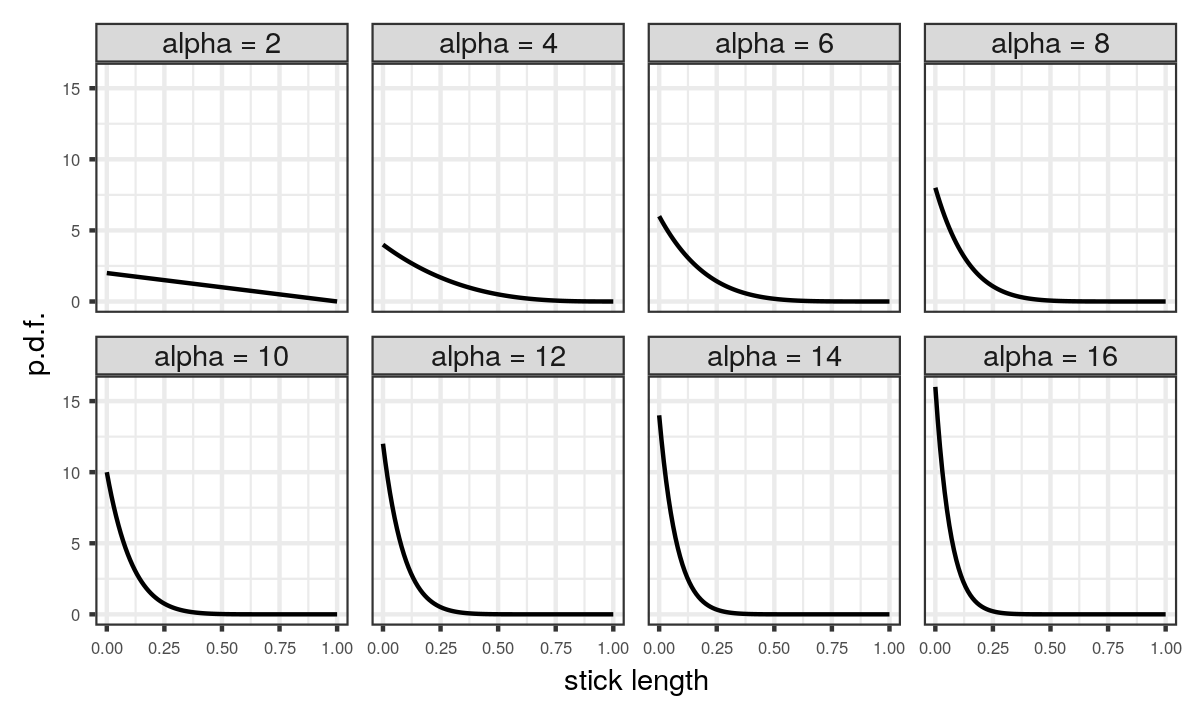
\includegraphics[width=0.980\linewidth,height=0.392\linewidth]{figure/beta_priors-1} 

}

\caption[Probability density functions of $\text{Beta}(1, \alpha)$ distributions, under various $\alpha$ considered for the iris data set]{Probability density functions of $\text{Beta}(1, \alpha)$ distributions, under various $\alpha$ considered for the iris data set.}\label{fig:beta_priors}
\end{figure}


\end{knitrout}



\begin{knitrout}
\definecolor{shadecolor}{rgb}{0.969, 0.969, 0.969}\color{fgcolor}\begin{figure}[!h]

{\centering 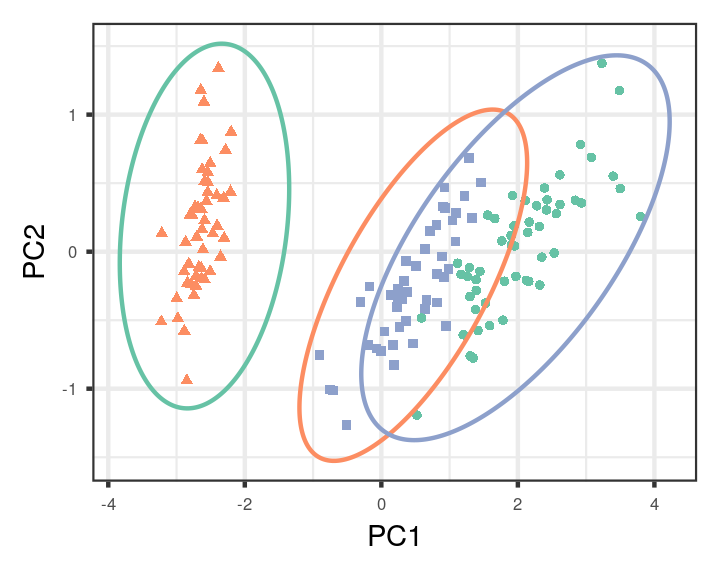
\includegraphics[width=0.588\linewidth,height=0.470\linewidth]{figure/iris_fit-1} 

}

\caption[The iris data in principal component space and
                      GMM fit at $\alpha = 2$]{The iris data in principal component space and
                      GMM fit at $\alpha = 2$. Colors denote inferred memberships and
                      ellipses represent estimated covariances. }\label{fig:iris_fit}
\end{figure}


\end{knitrout}
